%%%%%%%%%%%%%%%%%%%%%%%%%%%%%%%%%%%%%%%%%%%%%%%%%%%%%%%%%%%%%%%%%%%%%%%%%
\section{Additional Figures}  %%%%%%%%%%%%%%%%%%%%%%%%%%%%%%%%%%%%%%%%%%%
\label{rs:app:figures}

In this section, we present a few additional figures that complement the ones presented in Section~\ref{rs:sec:experiments} of the main text.

Figure~\ref{rs:fig:gifgif} presents the results on the GIFGIF dataset including a variant of uncertainty sampling.
This variant samples, at each iteration, $n-1$ comparisons consisting of adjacent pairs in the ranking $\hat{\bm{\theta}}$.
This strategy performs surprisingly poorly.

Figure~\ref{rs:fig:baselines2} presents results on synthetic datasets with $n = 200$ and $\lambda \in \{ 1, 2, 5, 10 \}$.
For the reader's convenience, we plot every graph on both a linear and a logarithmic scale.
Unsurprisingly, the gains of adaptive sampling are greater when the noise is smaller.

\begin{figure}[t]
\centering
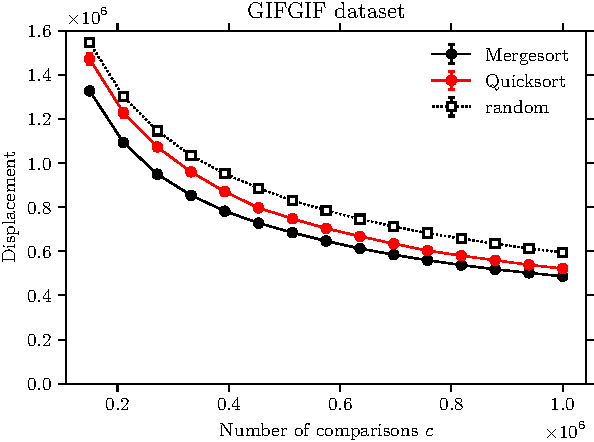
\includegraphics[width=0.67\linewidth]{rs-gifgif}
\caption{
Results on the GIFGIF dataset.
The experiment is repeated \num{10} times, and we report the mean and the standard deviation.
The variant of uncertainty sampling performs extremely poorly.
}
\label{rs:fig:gifgif}
\end{figure}


\begin{figure*}[t]
\centering
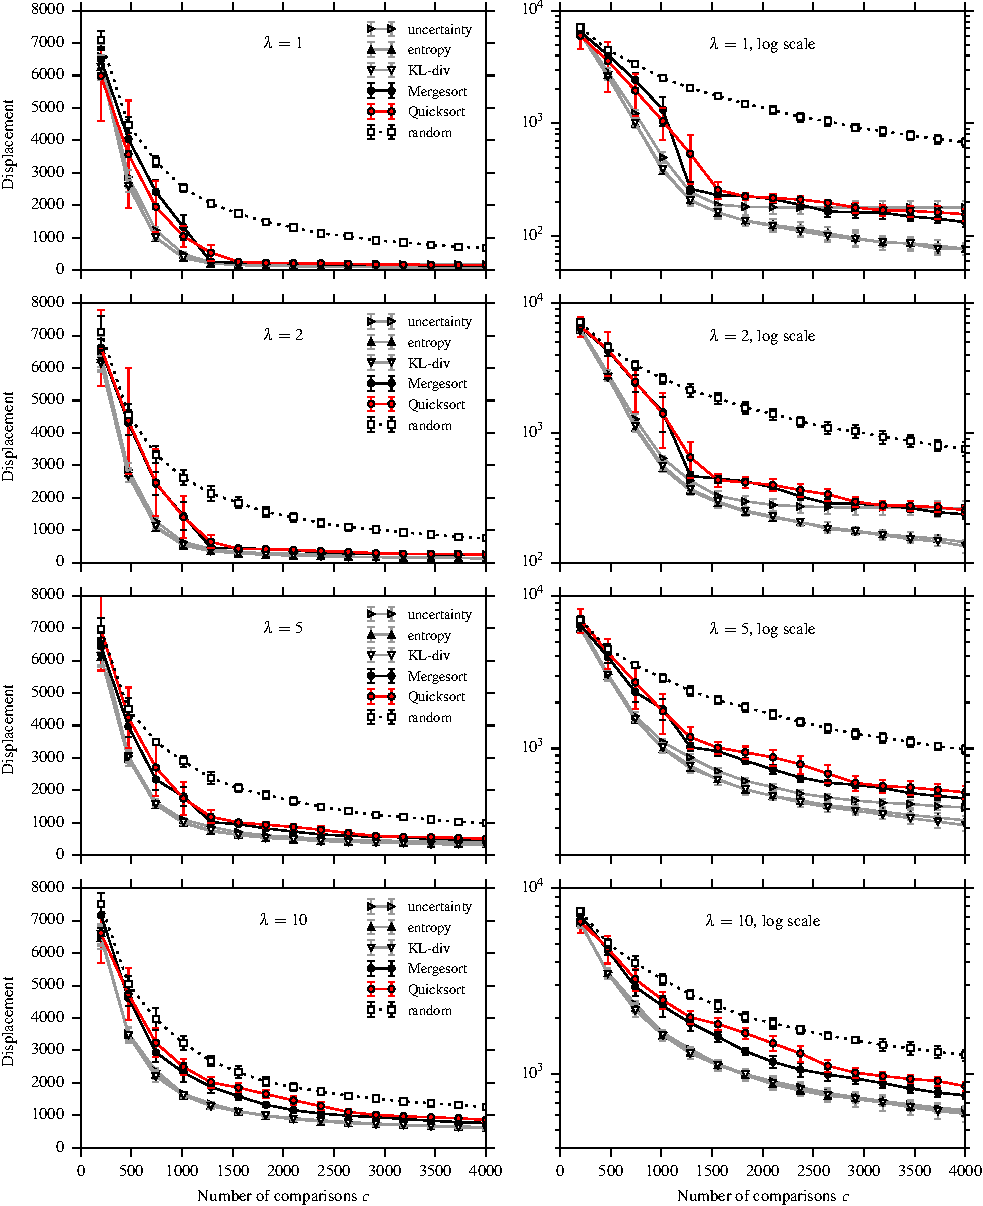
\includegraphics[width=\linewidth]{rs-baselines2}
\caption{
Results on synthetic datasets for $n = 200$ and increasing values of $\lambda$.
Every experiment is repeated \num{10} times, and we report the mean and the standard deviation.
}
\label{rs:fig:baselines2}
\end{figure*}
